\documentclass{article}
\usepackage{hyperref}
\usepackage{geometry}
\usepackage{amsmath}
\usepackage{amssymb}
\usepackage{graphicx}
\usepackage{algorithm}
\usepackage{algorithmic}
\usepackage{tcolorbox}
\usepackage{tikz}  
\usetikzlibrary{arrows.meta}
\usetikzlibrary{positioning}
\tikzset{>=stealth}

\definecolor{myblue}{rgb}{0.53, 0.94, 0.92}
\usepackage[bordercolor=black,
            linecolor=myblue,
            backgroundcolor=myblue,
            size=scriptsize]{todonotes}

\geometry{a4paper, scale=0.7}
\newtcolorbox{theorem}{colframe=red!75!black}
\newtcolorbox{proposition}{colframe=blue!75!black}
\newcommand{\x}{\mathbf{x}}
\newcommand{\X}{\mathbf{X}}
\newcommand{\s}{\mathbf{s}}
\newcommand{\I}{\mathbf{I}}
\newcommand{\w}{\mathbf{w}}

\title{Simulating infinite-dimensional diffusion bridges using score operator matching}
\author{Gefan Yang}
\begin{document}

\maketitle

\section{Introduction}
In the previous paper\cite{baker2024conditioning}, we discoverd the possibility of using Denoising Score Matching (DSM) to learn the score $\nabla p(x_t,t\mid x_0, 0)$ for non-linear diffusion process using the algorithm proposed by\cite{heng2022simulating}. However, we found that using only a fully-connected neural network to approximate high-dimensional score functions (more rigorously, the vector fields) can be nontrivial, specially when the learned objectives are Fourier coefficients of the score functions, the real and imaginary parts of coefficients need to be fed into the network individually as real vectors, which doubles the dimensions of the input and output. This drawback leads to the difficulty of scaling up the framework to high-dimensional cases. Besides that, since the shape is function in Hilbert spaces, the score should be defined in the context Hilbert spaces as well, which leads to the formulation of it as an operator that maps functions to functions, that is, we are going to match an operator.

Neural operators are proposed as a family of novel frameworks of neural network, which generalized the Universal Approximate Theorem of network over finite-dimensional spaces (values of functions) to infinite-dimensional function spaces. This formulation can overcome the inconsistency under different forms of discretization without additional training, and seems to show impressive performances on physical PDE solving. The essential idea behind neural operator is to formulate the unknown operator in terms of integral kernel operator. Depending on the choices of kernel function, typical neural operators are Graphic Neural Operator (GNO)\cite{li2020neural}, Low-rank Neural Operator (LNO)\cite{lu2021}, Multipole Graphic Neural Operator (MGNO)\cite{li2020multipole} and Fourier Neural Operator (FNO)\cite{li2021fourier}. In our case, we shall mainly focus on FNO, since we are also representing functions under Fourier basis, which coincides with the FNO framework.

In addition, we need to properly define the infinite-dimensional score as either operator or function (it turns out that these two are equivalent in the later discussion). Luckily, \cite{lim2023scorebased} has already given a well-defined form of infinite-dimensional DSM, we shall use their definition and combine with \cite{heng2022simulating}'s algorithm to develope a framework for infinite-dimensional diffusion bridge scheme.

\section{Background}
\subsection{Score-based diffusion model and diffusion bridge}
Score-matching techniques are initially developed to sample for generative purpose, i.e., sample from an unknown distribution, $p_{\text{data}}(\x)$, which is a marginal distribution at a certain time in the context of SDEs. However, in diffusion bridge simulation, we would like to sample from, essentially, a transition distribution or its variant. The latter is accessed by Doob's $h$-transform, as $h(\x, t):=\nabla_{\x(t)}\log q_{tT}(\x(T)\mid\x(t))$. In the rest of notes, we shall denote $q_{st}(\x(t)\mid\x(s))$ as the transition density from $\x(s)$ to $\x(t)$ for $0\leq s < t \leq T$. Therefore, it is necessary to think of what the objectives of the common score-based diffusion model are and how they can fit with our goals.

\subsubsection{Score-based diffusion generative models}
The essence of generative models is to approximate an unknown distribution $p_{\text{data}}(\x)$. In \cite{hyvarinen2005estimation}, the author first proposed the concept of ``score-matching'', which is commonly referred as implicit score matching in the later literatures
\begin{proposition}
    \textbf{Implicit score matching (ISM)}:
    \begin{equation} 
        L_{\text{ISM}}(\theta) := \mathbb{E}_{\x\sim p_{\text{data}}(\x)}\left[\frac{1}{2}\|\s_{\theta}(\x)\|^2_2 + \operatorname{tr}(\nabla_\x \s_{\theta}(\x)) \right] 
    \end{equation}
    For $\theta^* = \underset{\theta}{\arg\min} L_{\text{ISM}}(\theta)$, $\s_{\theta^*}(\x)\approx \nabla_\x\log p_{\text{data}}(\x)$.
\end{proposition}
Since ISM requires the gradient of $\s_{\theta}(\x)$, which is computationally costly. \cite{vincent2011connection} proposed the denoising score matching (DSM) approach, which is a gradient-free loss:
\begin{proposition}
    \textbf{Denoising score matching (DSM)}: Given the perturbation kernel $q_{\sigma}(\tilde{\x}\mid\x):=\mathcal{N}(\tilde{\x};\x,\sigma^2\I)$, and define $q_{\sigma}(\tilde{\x}):= \int q_{\sigma}(\tilde{\x}\mid\x)p_{\text{data}}(\x)d\x$,
    \begin{equation}
        L_{\text{DSM}}(\theta) := \frac{1}{2}\mathbb{E}_{\tilde{\x}\sim q_{\sigma}(\tilde{\x}\mid \x)} \mathbb{E}_{\x\sim p_{\text{data}(\x)}}\left[\| \s_{\theta}(\tilde{\x}) - \nabla_{\tilde{\x}}\log q_{\sigma}(\tilde{\x}\mid \x) \|^2_2\right] 
    \end{equation}
    For $\theta^* = \underset{\theta}{\arg\min} L_{\text{DSM}}(\theta)$, $\s_{\theta^*}(\x)\approx \nabla_\x\log q_{\sigma}(\x)$, and when $\sigma\to 0$, $q_{\sigma}(\x)\approx p_{\text{data}}(\x)$.
\end{proposition}
Then \cite{song2019generative} found that DSM suffers from poor approximations in the regions where the data is sparse, therefore, they proposed to perturb the data with different perturbation kernels $q_{\sigma_i}(\tilde{\x}\mid \x)$ instead of a fixed one, which leads to multi-level denoising score matching (they refer it as noise-condition score network (NCSN) in their paper)
\begin{proposition}
    \textbf{Multi-level denoising score matching (MDSM)}: Given perturbation kernels $q_{\sigma_i}(\tilde{\x}\mid\x):=\mathcal{N}(\tilde{\x};\x,\sigma_i^2\I)$ with a known sequence $\{\sigma_i\}_{i=1}^L$, where $\sigma_1 > \sigma_2 > \dots > \sigma_{L-1} > \sigma_L\approx 0$, and define $q_{\sigma_i}(\tilde{\x}):= \int q_{\sigma_i}(\tilde{\x}\mid\x)p_{\text{data}}(\x)d\x$
    \begin{equation}
        L_{\text{MDSM}}(\theta) := \frac{1}{L}\sum^L_{i=1}\lambda(\sigma_i)\mathbb{E}_{\tilde{\x}\sim q_{\sigma_i}(\tilde{\x}\mid \x)} \mathbb{E}_{\x\sim p_{\text{data}(\x)}}\left[\| s_{\theta}(\tilde{\x}, \sigma_i) - \nabla_{\tilde{\x}}\log q_{\sigma_i}(\tilde{\x}\mid \x) \|^2_2\right]
    \end{equation}
    For $\theta^* = \underset{\theta}{\arg\min} L_{\text{DSM}}(\theta)$ and $\forall\sigma\in\{\sigma_i\}_{i=1}^L$, $\s_{\theta^*}(\x, \sigma)\approx \nabla_\x\log q_{\sigma}(\x)$, and when $\sigma\to 0$, $q_{\sigma}(\x)\approx p_{\text{data}}(\x)$.
\end{proposition}
\cite{song2021scorebased} generalized the discrete multi-level perturbation into a continuous scenario, which leads to the formulation under the SDE framework.
\begin{proposition}
    \textbf{SDE Score matching (SDESM)}:
    Let $\x(t)$ be a random variable follows the SDE:
    \begin{equation} \label{eq: sde}
        d\x = f(\x, t)dt + g(\x, t)d\w
    \end{equation}
    and denote by $p_t(\x)$ the probability density of $\x(t)$ and use $q_{st}(\x(t)\mid\x(s))$ to denote the transition density as the statement before, and let $p_{\text{data}}(\x(0)) = p_{\text{data}}(\x)$.
    \begin{equation}
        \begin{split}
            L_{\text{SDE}}(\theta) := &\mathbb{E}_{t\sim\mathcal{U}(0, T)}\lambda(t)\mathbb{E}_{\x(t)\sim p_{0t}(\x(t)\mid \x(0))} \\
            &\mathbb{E}_{\x(0)\sim p_{\text{data}(\x(0))}}\left[\| \s_{\theta}(\x(t), t) - \nabla_{\x(t)}\log q_{0t}(\x(t)\mid \x(0)) \|^2_2\right]
        \end{split}
    \end{equation}
    For $\theta^* = \underset{\theta}{\arg\min} L_{\text{SDE}}(\theta)$, $\s_{\theta^*}(\x, t)\approx \nabla_\x \log p_t(\x)$.
\end{proposition}
Note that the connection between MDSM and SDESM is natural, since in SDESM, $p_t(\x) = \int q_{0t}(\x(t)\mid\x(0))p_{\text{data}}(\x(0))d\x(0)$, which aligns with the definition in MDSM. We can see that \emph{the score-matching techniques can only approximate the transition density from before to current moment.} While in the bridge simulation, we require the transition density from the future to current moment.

If the drift term $f(\cdot, t)$ in \ref{eq: sde} is affine and the diffusion term $g(\cdot, t) = g(t)$ is linear, the transition density $p_{st}(\x(t)\mid\x(s))$ are always Gaussian and therefore $\nabla_{\x(t)}\log q_{0t}(\x(t)\mid \x(0))$ has a close form. For more general cases, \cite{heng2022simulating} extends it to nonlinear cases. \todo{Suspicious, should it be $\nabla_{\x}\log p_t(\x)$ here as before? Does it imply that $p(\x(0))=1$?}
\begin{theorem}
    \textbf{Nonlinear SDE Score matching (NSDESM)}: For any partition $\{t_m\}_{m=0}^M$ of the interval $[0, T]$, the loss function is defined as:
    \begin{equation}
        \begin{split}
            L_{NSDE}(\theta) := \frac{1}{2}\sum^M_{m=1}\int^{t_m}_{t_{m-1}}&\mathbb{E}_{\x(0)\sim p_{\text{data}}(\x(0))}\big[\| \s_{\theta}(\x(t), t) \\
            &- \nabla_{\x(t)}\log q_{t_{m-1}t}(\x(t)\mid\x(t_{m-1})) \|^2_{g^2(\x(t),t)}\big]dt
        \end{split}
    \end{equation}
    For $\theta^* = \underset{\theta}{\arg\min} L_{\text{NSDE}}(\theta)$, $\s_{\theta^*}(\x, t)\approx \nabla_\x\log q_{0t}(\x\mid\x(0))$. 
\end{theorem}


\begin{figure}[H]
    \centering
    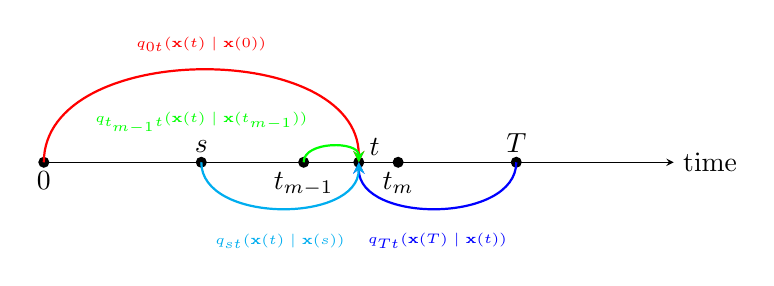
\begin{tikzpicture}
        \centering
        \draw[->,line width=0.2pt](0.0,0)--(8.0,0) node[right] {time};
        \coordinate (a) at position (0.0, 0);
        \coordinate (b) at position (2.0, 0);
        \coordinate (c) at position (4.0, 0);
        \coordinate (d) at position (6.0, 0);
        \coordinate (e) at position (3.3, 0);
        \coordinate (f) at position (4.5, 0);
        \fill (0.0, 0) circle (2pt) node[below] {$0$};
        \fill (6.0, 0) circle (2pt) node[above] {$T$};
        \fill (2.0, 0) circle (2pt) node[above] {$s$};
        \fill (4.0, 0) circle (2pt) node at (4.2, 0.2) {$t$};
        \fill (3.3, 0) circle (2pt) node[below] {$t_{m-1}$};
        \fill (4.5, 0) circle (2pt) node[below] {$t_{m}$};

        \draw[red, ->, thick] (a.90) to[in=90, out=90] (c.90) node at (2.0, 1.5) {\tiny $q_{0t}(\x(t)\mid\x(0))$};  
        \draw[blue, ->, thick] (d.0) to[in=-90, out=-90] (c.0) node at (5.0, -1.0) {\tiny $q_{Tt}(\x(T)\mid\x(t))$};
        \draw[cyan, ->, thick] (b.0) to[in=-90, out=-90] (c.0) node at (3.0, -1.0) {\tiny $q_{st}(\x(t)\mid\x(s))$};
        \draw[green, ->, thick] (e.0) to[in=90, out=90] (c.0) node at (2.0, 0.5) {\tiny $q_{t_{m-1}t}(\x(t)\mid\x(t_{m-1}))$};
    \end{tikzpicture}
\end{figure}


\cite{anderson1982reverse} shows an important theorem of the time-reversed SDE of a given SDE
\begin{theorem}
    \textbf{Anderson's time-reversed diffusion theorem}: Let $X_t$ be a stochastic process described by the SDE:
    \begin{equation}
        d\x = f(\x,t)dt + g(\x, t)d\w
    \end{equation}
    The reverse time model for $\x(t)$ is:
    \begin{equation}
        d\x = \bar{f}(\x, t)dt + g(\x, t)d\bar{\w}
    \end{equation}
    where,
    \begin{equation}
        \bar{f}(\x, t) = f(\x, t) - \frac{1}{p_t(\x)}\nabla_{\x}[p_t(\x)g(\x, t)g^T(\x, t)]
    \end{equation}
    and $p_t(\x):= \int q_{0t}(\x(t)\mid\x(0))p(\x(0))d\x(0)$ as defined above.
\end{theorem}


\subsection{Diffusion shape process in function spaces}
We are more interested in the diffusion bridge process of shape evolution, i.e, how the shapes evolve stochastically along with time, and especially, it should be conditioned on hitting a target shape (or surroundings with infinitesimal distances) within finite time. Rigorously, a shape $\mathcal{S}$ is usually treated as a function from an underlying manifold $\mathcal{M}$ to Euclidean space $\mathbb{R}^d$ and two shapes $\mathcal{S}, \mathcal{S}'$ are equivalent up to a representation if there exists a diffeomorphism $\phi\in\operatorname{Diff}(\mathcal{M})$ such that $\mathcal{S} = \mathcal{S}'\circ\phi$\cite{baker2023function}. Suppose we have a finite collection of observations of $\mathcal{S}$ in $\mathbb{R}^d$, denote as $s^{(1)},\dots,s^{(N)}, s^{(i)}\in\mathbb{R}^d$, which are often referred as \emph{landmarks}. Given the landmark representations of initial shape $\mathcal{S}_i$ and target shape $\mathcal{S}_t$, $s_i\in\mathbb{R}^{N\times d}$ and $s_t\in\mathbb{R}^{N\times d}$, the difference $x = s_t-s_i \in \mathbb{R}^{N\times d}$ are the $N$ observations of a function $X\in L^2(\mathcal{M},\mathbb{R}^d)$. Take the time into account and $X_t\in L^2(\mathcal{M}\times[0, T], \mathbb{R}^d)$. We can also defined an unconditional SDE for functions in Hilbert spaces, which follows similarly from:
\begin{equation}
    dX_t = F(X_t, t)dt + B(X_t, t)dW_t, 
\end{equation}
and apply infinite-dimensional Doob's $h$-transform\cite{baker2024conditioning} to get the conditional SDE:
\begin{equation}
    dX^*_t = \{F(X^*_t, t) + B(X^*_t, t)B^*(X^*_t, t)\nabla\log h(X^*_t,t)\}dt + B(X^*_t, t)dW_t
\end{equation}
where $h: H\times [0, T]\to\mathbb{R}$ and $\nabla\log h: H\times[0, T]\to H$, we refer the latter as the \emph{score operator}. We further show that under a certain choice of basis of $H$, a finite collection of the projections of $\nabla\log h$, denote as $(\nabla\log h)_N$ is a real-valued function that maps $H_N\times[0, T]\to\mathbb{R}^N$, where $H_N$ is a subspace of $H$ with the dimension of $N$, which is essentially $\mathbb{R}^N$, so it would make sense to match the first $N$ components of $\nabla\log h$ as real functions between Euclidean spaces. However, in the further discussion, we will see it is possible to directly matching the infinite-dimensional score operator without projecting it into finite dimensional spaces, which requires the framework of neural operators.

\subsection{Fourier neural operator}
\textbf{Neural operator formulation}: Neural operators are designed to learn a mapping between two infinite dimensional spaces by using a finite collection of observations of input-output pairs from this mapping. Let $\mathcal{A}$ and $\mathcal{U}$ be Banach spaces of functions defined on bounded domains $D\subset \mathbb{R}^d$ and $D'\subset\mathbb{R}^{d'}$. The neural operator $\mathcal{G}_{\theta}$ is a parametric approximation of $\mathcal{G}_{\dagger}:\mathcal{A}\to\mathcal{U}$. Given the input function $a\in\mathcal{A}$ are $\mathbb{R}^{d_a}$-valued and output function $u\in\mathcal{U}$ are $\mathbb{R}^{d_u}$-valued. The neural operator is constructed as followed\cite{kovachki2023neural}:
\begin{enumerate}
    \item \textbf{Lifting} ($\mathcal{Q}:\mathbb{R}^{d_a}\to\mathbb{R}^{d_{v_0}}$): Map the input $\{a:D\to\mathbb{R}^{d_a}\} \mapsto \{v_0: D\to \mathbb{R}^{d_{v_0}}\}$ to its first hidden representation, by choosing $d_{v_0} > d_a$, $\mathcal{Q}$ is a lifting operator.
    \item \textbf{Iterative Kernel Integration}: For each layer index by $l=0,1,\dots,L-1$, map each hidden representation from last layer to the next $\{v_l:D_l\to\mathbb{R}^{d_{v_l}}\}\mapsto\{v_{l+1}:D_{l+1}\to\mathbb{R}^{d_{v_{l+1}}}\}$ via the action of the sum of a local linear operator (matrix) $W_l\in\mathbb{R}^{d_{v_{l+1}}\times d_{v_l}}$, a non-local integral kernel operator $\mathcal{K}_l:\{v_l:D_l\to\mathbb{R}^{d_{v_l}}\}\mapsto\{v_{l+1}:D_{l+1}\to\mathbb{R}^{d_{v_{l+1}}}\}$, and a bias function $b_l:D_l\to\mathbb{R}^{d_{v_{l+1}}}$, where $D_0=D, D_{L}=D'$, and activated by a nonlinear function $\sigma_l: \mathbb{R}^{d_{v_{l+1}}}\to\mathbb{R}^{d_{v_{l+1}}}$.
    \item \textbf{Projection} ($\mathcal{P}:\mathbb{R}^{d_{v_{L}}}\to\mathbb{R}^{d_u}$): Map the last hidden representation $\{v_L:D'\to\mathbb{R}^{d_{v_L}}\} \mapsto \{u: D'\to \mathbb{R}^{d_{u}}\}$ to the output function, by choosing $d_{v_L}>d_{u}$, $\mathcal{P}$ is a projection map.
\end{enumerate}
In summary, the above description can be represented using a single formulation:
\begin{equation} \label{eq: neural operator}
    \mathcal{G}_{\theta} := \mathcal{P}\circ \sigma_L(W_{L-1}+\mathcal{K}_{L-1}+b_{L-1})\circ\dots\circ\sigma_1(W_0+\mathcal{K}_0+b_0)\circ\mathcal{Q}
\end{equation}

The essence of neural operators is the integral kernel operator $\mathcal{K}_l$, as defined as followed:
\begin{equation} \label{eq: integral kernel op}
    (\mathcal{K}_l(v_l))(x) = \int_{D_l}\kappa^{(l)}(x, y)v_l(y)d\nu_l(v),\quad \forall x\in D_{l+1}
\end{equation}
where $\kappa^{(l)}:D_{l+1}\times D_{l}\to\mathbb{R}^{d_{v_{l+1}}\times d_{v_l}}$ and $\nu_l$ is usually chosen as the Lebesgue measure on $\mathbb{R}^{d_l}$.

\noindent\textbf{Fourier neural operator}: Let's focus on a specific layer and omit the index $l$ and assume $d\nu(y)=dy$. Then \ref{eq: integral kernel op} gives the update of a single layer:
\begin{equation}
    u(x) = \int_D \kappa(x, y)v(y)dy,\quad \forall x\in D
\end{equation}
Let $D=\mathbb{T}^d$ is the unit torus and $\mathcal{F}:L^2(D;\mathbb{C}^{d_v})\to\ell^2(\mathbb{Z}^d;\mathbb{C}^{d_v})$ be the Fourier transform of a complex-valued function $v:D\to\mathbb{C}^{d_v}$ and $\mathcal{F}^{-1}$ be its inverse, for $v\in L^2(D;\mathbb{C}^{d_v})$ and $w\in\ell^2(\mathbb{Z}^d;\mathbb{C}^{d_v})$, we have:
\begin{align}
    &(\mathcal{F}v)_j(k) = \langle v_j, \psi_k \rangle_{L^2(D;\mathbb{C})},\quad j\in\{1,\dots,n\},k\in\mathbb{Z}^d \label{eq: fwd fourier}
    \\
    &(\mathcal{F}^{-1}w)_j(x) = \sum_{k\in\mathbb{Z}^d}w_j(k)\psi_k(x),\quad j\in\{1,\dots,n\},x\in D \label{eq: bwd fourier}
\end{align}
where, for each $k\in\mathbb{Z}^d$, define,
\begin{align}
    \psi_k: D &\to \mathbb{C} \\
    x &\mapsto\exp(-i2\pi(k_1x_1+\dots+k_dx_d))
\end{align}
By letting $\kappa(x, y) = \kappa(x-y)$ for some periodic function $\kappa: D\to \mathbb{C}^{d_u\times d_v}$ and applying convolution theorem, we find:
\begin{equation}
    u(x) = \mathcal{F}^{-1}(\mathcal{F}(\kappa)\cdot \mathcal{F}(v))(x),\quad \forall x\in D
\end{equation}
Therefore, we shall directly parametrize $\kappa$ by its Fourier coefficients:
\begin{equation} \label{eq: fourier integral}
    u(x) = \mathcal{F}^{-1}(R_\phi\cdot \mathcal{F}(v))(x),\quad x\in D
\end{equation}
For each frequency mode $k\in\mathbb{Z}^d$, we have $\mathcal{F}(\kappa)(k) = R_\phi(k)\in\mathbb{C}^{d_u\times d_v}$, that is, for each $k$, $R_\phi(k)$ is a $d_u\times d_v$ complex matrix. We pick a finite-dimensional collection of frequency modes by truncating the Fourier series at a maximal number of modes $k_{\max} = \left\lvert Z_{k_{\max}}\right\rvert = \left\lvert \{k\in\mathbb{Z}^d: \left\lvert k_j \right\rvert \leq (\mathfrak{k}_{\max})_j, j=1,\dots,d, \mathfrak{k}_{\max}\in\mathbb{Z}_{+}^d\}\right\rvert $, then we can parametrize $R_\phi$ directly as a $k_{\max}\times d_u\times d_v$ complex tensor and therefore drop off the parameter $\phi$. The actual form of $R$ depends on the choice of periodic function $\kappa$. In addition, if the mapping happens between the real-valued functions, we shall impose that $\kappa$ is also real-valued by enforcing conjugate symmetry in the parameterization, i.e.
\begin{equation}
    R(-k)_{m,n} = R^*(k)_{m, n}, \quad \forall k\in Z_{k_{\max}}\subset\mathbb{Z}^d,\quad m=1,\dots,d_u, \;n=1,\dots,d_v
\end{equation}
A pictorial representation of FNO is shown in \ref{fig: FNO}
\begin{figure} \label{fig: FNO}
    \centering
    \includegraphics[width=0.8\textwidth]{figures/FNO.png}
    \caption{(a) The overall architecture of Fourier Neural Operator; (b) The detailed Fourier layer}
\end{figure}

\noindent\textbf{Discrete case and FFT}: The content above is the continuous case, we shall talk about the discrete implementation of FNO and apply FFT to accelerate the Fourier transformation. Let the domain $D$ be discretized into $N\in\mathbb{N}$ points with resolution of $N_1\times\dots\times N_d$ for $N_1,\dots,N_d\in\mathbb{N}$ and $\prod_{i=1}^d N_i=N$. Then we shall treat $v\in\mathbb{C}^{N_1\times\dots\times N_d\times d_v}$ and $\mathcal{F}(v)\in\mathbb{C}^{N_1\times\dots\times N_d\times d_v}$. Suppose we truncate at the position $Z_{k_{\max}}\in\mathbb{Z}^d$, and leave a subtensor of $\mathcal{F}(v)\in\mathbb{C}^{(\mathfrak{k}_{\max})_1\times\cdots\times (\mathfrak{k}_{\max})_d\times d_v}$. We also truncate the Fourier coefficients of the kernel $\kappa$ in the same way, that is, $R = \mathcal{F}(\kappa)\in\mathbb{C}^{(\mathfrak{k}_{\max})_1\times\cdots\times (\mathfrak{k}_{\max})_d\times d_u\times d_v}$. The weighted multiplication in \ref{eq: fourier integral} can be written as:
\begin{align}
    (R\cdot \mathcal{F}(v))_{k_1,\dots,k_d,m} &= \sum^{d_v}_{n=1}R_{k_1,\dots,k_d,m,n}(\mathcal{F}(v))_{k_1,\dots,k_d,n}, \label{eq: kernel multi}\\
    k_j &= 1,\dots,(\mathfrak{k}_{\max})_j\text{ for } j=1, \dots, d; \\
    m &= 1,\dots,d_u
\end{align}
In the above multiplication, $\mathcal{F}(v)$ can be efficiently computed by $d$-dimensional DFT if the discretization is uniform. For $v\in\mathbb{C}^{N_1\times\dots\times N_d\times d_v}$, $k=(k_1,\dots,k_d)\in\mathbb{Z}_{N_1}\times\dots\times\mathbb{Z}_{N_d}$, and $x=(x_1,\dots,x_d)\in D$, the $d$-dimensional DFT $\hat{\mathcal{F}}$ and its inverse $\hat{\mathcal{F}}^{-1}$ are defined as:
\begin{align}
    (\hat{\mathcal{F}}v)(k) &= \sum_{n_1=0}^{N_1}\dots\sum_{n_d=1}^{N_d}v_{n_1,\dots,n_d}\exp(-2i\pi\sum_{j=1}^{d}\frac{x_j}{N_j}k_j) \label{eq: ndim DFT}\\
    (\hat{\mathcal{F}}^{-1}v)(x) &= \sum_{n_1=0}^{N_1}\dots\sum_{n_d=1}^{N_d}v_{n_1,\dots,n_d}\exp(2i\pi\sum_{j=1}^{d}\frac{k_j}{N_j}x_j) \label{eq: ndim iDFT}
\end{align}
Both \ref{eq: ndim DFT} and \ref{eq: ndim iDFT} can be computed via Fast Fourier Transform (FFT). Note that when truncate the Fourier domain, the sum bound in \ref{eq: ndim iDFT} will end up to $Z_{k_{\max}}$ instead of $N$, and the truncation in this case is taking the "corner" of $(\mathcal{F}(v))$, which is similar to the computation of $R$.

\noindent\textbf{Choice for $R$}: In general, $R$ should be defined to depend on $\mathcal{F}(a)$, the Fourier transform of the input $a\in\mathcal{A}:D\to\mathbb{C}^{d_a}$, we shall define $R_\phi:\mathbb{Z}^d\times\mathbb{C}^{d_a}\to\mathbb{C}^{d_u\times d_v}$ as a parametric function that maps $(k, (\mathcal{F}(a))(k))$ to the Fourier coefficients of the appropriate Fourier modes, in \cite{kovachki2023neural}, they proposed three choices of $R_\phi$:
\begin{itemize}
    \item \textit{direct parameterization}: Define the parameters $\phi_k\in\mathbb{C}^{d_u\times d_v}$ for each wave number $k\in\mathbb{N}$:
    \begin{equation}
        R_\phi(k, (\mathcal{F}(a))(k)) := \phi_k
    \end{equation}
    \item \textit{linear parameterization}: Define the parameters $\phi_{k_1}\in\mathbb{C}^{d_u\times d_v\times d_a}, \phi_{k_2}\in\mathbb{R}^{d_u \times d_v}$, for each wave number $k\in\mathbb{N}$:
    \begin{equation}
        R_\phi(k, (\mathcal{F}(a))(k)) := \phi_{k_1}(\mathcal{F}(a))(k) + \phi_{k_2}
    \end{equation}
    \item \textit{feed-forward neural network}: Let $\Phi_\phi: \mathbb{Z}^d\times\mathbb{C}^{d_a} \to \mathbb{C}^{d_u\times d_v}$ be a neural network with parameters $\phi$:
    \begin{equation}
        R_\phi(k, (\mathcal{F}(a))(k)) := \Phi_\phi(k, (\mathcal{F}(a))(k))
    \end{equation}
\end{itemize}
In summary, the algorithm of computing Fourier layer is summarized in \ref{alg: fourier layer}. Empirically, the direct and linear parameterization have similar performances and the feed-forward network has the worst one. Besides, the direct parameterization has the simplest computation complexity and least parameters required.
\begin{algorithm}
    \renewcommand{\algorithmicrequire}{\textbf{Input:}}
    \renewcommand{\algorithmicensure}{\textbf{Output:}}
    \caption{Fourier layer}
    \label{alg: fourier layer}
    \begin{algorithmic}
        \REQUIRE $v\in\mathbb{C}^{N_1\times\dots\times N_d\times d_v},\; R\in\mathbb{C}^{N_1\times\dots\times N_d\times d_u\times d_v},\; W\in\mathbb{C}^{d_u\times d_v},\;b\in\mathbb{C}^{d_u}$
        \STATE $\tilde{v} = \hat{\mathcal{F}}(v) \in \mathbb{C}^{N_1\times\dots\times N_d\times d_v}$ by \ref{eq: ndim DFT};
        \STATE Truncate $\tilde{v}$ at $Z_{k_{\max}}$, obtain $\tilde{v}'\in \mathbb{C}^{(\mathfrak{k}_{\max})_1\times\dots\times (\mathfrak{k}_{\max})_d\times d_v}$;
        \STATE $\tilde{v}' = R\cdot\tilde{v}' \in \mathbb{C}^{(\mathfrak{k}_{\max})_1\times\dots\times (\mathfrak{k}_{\max})_d\times d_u}$ by \ref{eq: kernel multi};
        \STATE $u = \hat{\mathcal{F}}^{-1}(\tilde{v})$ by \ref{eq: ndim iDFT};
        \STATE $u = \sum_{j=1}^{d_u}(u_{\dots,j}W_{j,\dots} + b_{j})$;
        \STATE $u = \sigma(v)$
        \ENSURE $u\in \mathbb{C}^{(\mathfrak{k}_{\max})_1\times\dots\times (\mathfrak{k}_{\max})_d\times d_u}$
    \end{algorithmic}
\end{algorithm}

\subsection{Infinite-dimensional score matching}
\subsubsection{Define infinite-dimensional score}
Now back to our shape problem, we would like to model the stochastic evolution of the displacement function $X: \mathcal{M}\to\mathbb{R}^d$, let the shape defined in $\mathbb{R}^2$, $\mathcal{M}$ be the interval $[-\pi, \pi]$ with periodic boundaries, that is, $X:[-\pi, \pi]\to\mathbb{R}^2$. If in finite-dimensional case, the score $s$ is defined as a vector field that maps $\mathbb{R}^d\to\mathbb{R}^d$. While in the infinite case, $s$ is an operator that maps between Hilbert spaces. \cite{lim2023scorebased} dedicated to define such a score operator denoted by:
\begin{equation}
    D_{H_{\mu_0}}\Phi = D_{H_{\mu_0}}\log\frac{d \nu}{d\mu_0},\quad D_{H_{\mu_0}}\Phi: H\to H^*_{\mu_0}
\end{equation}
where $\Phi:H\to\mathbb{R}$ is a Fréchet differentiable Borel measurable mapping, $H_{\mu_0}$ is Cameron-Martin space, which itself is a Hilbert space, $\nu$ is the the probability measure induced by the function perturbation 
\begin{equation} \label{eq: data perturb}
    v = u + \eta, \quad u\sim \mu, \;\eta\sim \mu_0,\; u,\eta\in H
\end{equation}
$D_{H_{\mu_0}}$ is the Fréchet derivative and $\Phi$ suffices:
\begin{equation}
    \frac{d\nu}{d\mu_0}(w) = \exp(\Phi(w)),\quad \mu_0\text{-a.s.},\; w\in H
\end{equation}
The \emph{infinite-dimensional score} of $\nu\in H$ is $D_{H_{\mu_0}}\Phi: H\to H^*_{\mu_0}$, which is a mapping between Hilbert spaces, therefore is an \emph{operator}, in the following text, we shall call it \emph{score} for short. 

\subsubsection{Denoising score matching}
Let $\mathcal{G}_\theta:H\to H^*_{\mu_0}$ be the parametric mapping and then the score matching loss is:
\begin{equation}
    \underset{\theta}{\min}\mathbb{E}_{v\sim\nu}\left\lVert D_{H_{\mu_0}}\Phi(v) - \mathcal{G}_{\theta}(v)\right\rVert^2_{H^*_{\mu_0}},\quad v\in H 
\end{equation}
which is intractable to compute and the denoising score matching scheme needs to be applied. Consider the Gaussian transition of $v\mid u$, $\mathcal{N}(u, C):=\gamma^u$ for $\mu$-almost any $u\in H$, where $C:H\to H$ is the covariance operator. For $\mu_0$-almost any $w\in H$ and $\mu$-almost any $u\in H_{\mu_0}$,
\begin{equation}
    \frac{d\gamma^u}{d\mu_0}(w) = \exp\left(\sum_{j=1}^{\infty}\lambda^{-1}_j\left\langle w,\varphi_j\right\rangle \left\langle u, \varphi_j\right\rangle - \frac{1}{2}\left\lVert C^{-1/2}(u)\right\rVert^2  \right) := \exp(\Psi(w;u))
\end{equation}
where $C\varphi_j = \lambda_j\varphi_j$ is the eigendecomposition of $C$. The score of each conditional $\gamma^u$ is given as the Fréchet derivative of the \emph{potential} $\Psi: H\times H_{\mu_0}\to\mathbb{R}$ in the direction of $H_{\mu_0}$, then the \emph{infinite-dimensional denoising score matching} loss is:
\begin{equation}
    \underset{\theta}{\min} \mathbb{E}_{u\sim\mu}\mathbb{E}_{w\sim\gamma^u}\left\lVert D_{H_{\mu_0}}\Psi(w;u) - \mathcal{G}_\theta(w)\right\rVert^2_{H^*_{\mu_0}}, \quad u\in H_{\mu_0},\; w\in H. 
\end{equation}
The first term in inf-dim DSM can be computed by
\begin{equation}
    D_{H_{\mu_0}}\Psi(w;u) = \sum_{j=1}^{\infty}\lambda^{-1}_j\left\langle u,\varphi_j\right\rangle \varphi_j,\quad D_{H_{\mu_0}}\Psi: H\times H_{\mu_0}\to H^*_{\mu_0}
\end{equation}
Furthermore, for $z\in H_{\mu_0}$,
\begin{equation}
    D_{H_{\mu_0}}\Psi(w;u)(z) = \sum_{j=1}^{\infty}\lambda^{-1}_j\left\langle z,\varphi_j\right\rangle \left\langle u, \varphi_j\right\rangle
\end{equation}
Since in, the ``score'' $s(X^*_t, t)$ should be also a function in $H$ in the context of $X^*\in H$, while the learned $\mathcal{G}_\theta$ lives in the dual space. In order to derive a form that lives in $H$ as well, the \emph{Riesz representation theorem} shall be applied:

\begin{theorem}
    \noindent\textbf{Riesz representation theorem}: Let $H$ be a Hilbert space equipped with inner product $\left\langle \cdot,\cdot\right\rangle:H\times H\to\mathbb{R}$. For every continuous linear function $\varphi\in H^*$, there exists a unique vector $f_\varphi \in H$, s.t.
\begin{equation}
    \varphi(x) = \left\langle x, f_\varphi\right\rangle, \quad \forall x\in H 
\end{equation} 
and the map $R:\varphi\mapsto f_\varphi, H^*\to H$, is a canonical isometric isomorphism.
\end{theorem}

By applying the Reisz map $R$ on $\mathcal{G}_\theta$, we obtain the operator $R\mathcal{G}_{\theta}:H\to H$, also using the isometric property (distance preserving), we find:
\begin{equation}
    \left\lVert D_{H_{\mu_0}}\Psi(v;u) - \mathcal{G}_\theta(v)\right\rVert^2_{H^*_{\mu_0}} = \left\lVert C^{-1/2}(u-R\mathcal{G}_\theta(v))\right\rVert^2_{H_{\mu_0}},\quad v\in H, u\in H_{\mu_0} 
\end{equation}
where in the R.H.S, the norm is taken in $H_{\mu_0}$ instead of $H^*_{\mu_0}$. And finally, the simpler inf-dim DSM loss is:
\begin{equation} \label{eq: inf-dim dsm}
    \underset{\theta}{\min}\mathbb{E}_{u\sim\mu}\mathbb{E}_{\eta\sim\mu_0}\left\lVert C^{-1/2}(u-R\mathcal{G}_\theta(u+\eta))\right\rVert^2 
\end{equation}
which is the infinite-dimensional analog to the original DSM loss in \cite{vincent2011connection}:
\begin{equation}
    \underset{\theta}{\min}\mathbb{E}_{x\sim p(x)}\mathbb{E}_{\eta\sim\mathcal{N}(0, \sigma^2I)}\left\lVert \frac{\eta}{\sigma^2} + s_\theta(x+\eta)\right\rVert^2_2
\end{equation}

\subsubsection{Data perturbation}
\ref{eq: data perturb} shows the general form of perturbing function data. In \cite{lim2023scorebased}, the author propose to perturb the data by structured noise instead of purely independent white noise, which is available as a \emph{Gaussian process}, also called \emph{Gaussian random field (GRF)} in some cases. Mathematically, a Gaussian process is defined as:
\begin{theorem}
    \noindent\textbf{Gaussian process $\operatorname{GP}$}: Let $X$ be a set, and let $f:X\to\mathbb{R}$ be a random function. We say that $f\sim\operatorname{GP}(\mu, k)$ if for any $n\in\mathbb{N}$ and any finite set of points $\mathbf{x}\in X^n$, the random vector $\mathbf{f}=f(\mathbf{x})\in\mathbb{R}^n$ is $n$-dimensional multivariate Gaussian with prior mean vector $\mathbf{\mu}=\mu(\mathbf{x})\in\mathbb{R}^n$ and covariance matrix $\mathbf{K}_{\mathbf{xx}} = k(\mathbf{x}, \mathbf{x})$. The function $k:\mathbb{R}^n\times\mathbb{R}^n\to\mathbb{R}$ is called the \emph{kernel} of Gaussian process.
\end{theorem}
A Gaussian process is uniquely determined by the mean function $\mu:X\to\mathbb{R}$ and the kernel function $k:X\times X\to\mathbb{R}$. There are many different choices of kernels, including two commonly used ones: Matérn-type kernel and radius basis function, they are defined as followed:
\begin{align}
    k_{\text{Matérn}}(x, x';\sigma, \kappa, \nu) &= \sigma^2\frac{2^{1-\nu}}{\Gamma(\nu)}\left(\sqrt{2\nu}\frac{\| x-x' \|}{\kappa}\right)^\nu K_{\nu}\left(\sqrt{2\nu}\frac{\| x-x' \|}{\kappa}\right) \\
    k_{\text{RBF}}(x, x';\sigma, \kappa) &= \sigma^2\exp\left(-\frac{\| x - x' \|^2}{2\kappa^2}\right)
\end{align}
The RBF can be treated as the limit of Matérn kernel as $\nu\to\infty$. There are many ways to sample from a GP, we here so far use the simplest and most intuitive way: Cholesky decomposition \todo{Maybe use different efficient methods, like the discrete convolution.}, essentially, it computes the square root of the covariance matrix computed by the kernel, which is the standard deviation, and multiply this on a discrete white noise field.

\section{Research problems}
The ultimate goal of this project is to \emph{simulate the diffusion bridge of infinite-dimensional shape displacements}. In order to achieve this, we need to address the following issues:
\begin{itemize}
    \item \textbf{Implement Fourier neural operator} Neural operators were initially developed for solving PDEs and there seems no usable implementation of score operator matching (in \cite{lim2023scorebased} used FNO but they didn't provide the source code). Also, the most comprehensive neural operator code base is \href{https://github.com/neuraloperator/neuraloperator}{neuraloperator} which is written in PyTorch. A good start shall be rewriting it using JAX, but for some very simple demos, to get some experiences on the implementation side, especially the computation of loss functions. After getting know about how exactly it works, we then develope the structure used for our purpose.
    \item \textbf{Derive the inf-dim DSM loss for the transition density of bridge} is the generalization of original DSM (matching normal density) to bridges (matching transition density), while is also used to match normal ``density'' of functions, we need to derive the corresponding variation of matching the ``transition density'' of the functions as well.
    \item \textbf{Add additional conditions to the score approximator} The existing framework only allows us to bridge a single pair of points, to bridge other pairs requires additional training. We could incorporate extra condition into the network, for example, $s_\theta(x_t, x_0, t)$, just like conditional diffusion model, to generalize to different bridges without extra training.
\end{itemize}

\bibliographystyle{plain}
\bibliography{refs}

\end{document}

